\author{Thijs Heus}
\lecture{Overview of UCLA LES}{overview}
\begin{frame}{This Week}
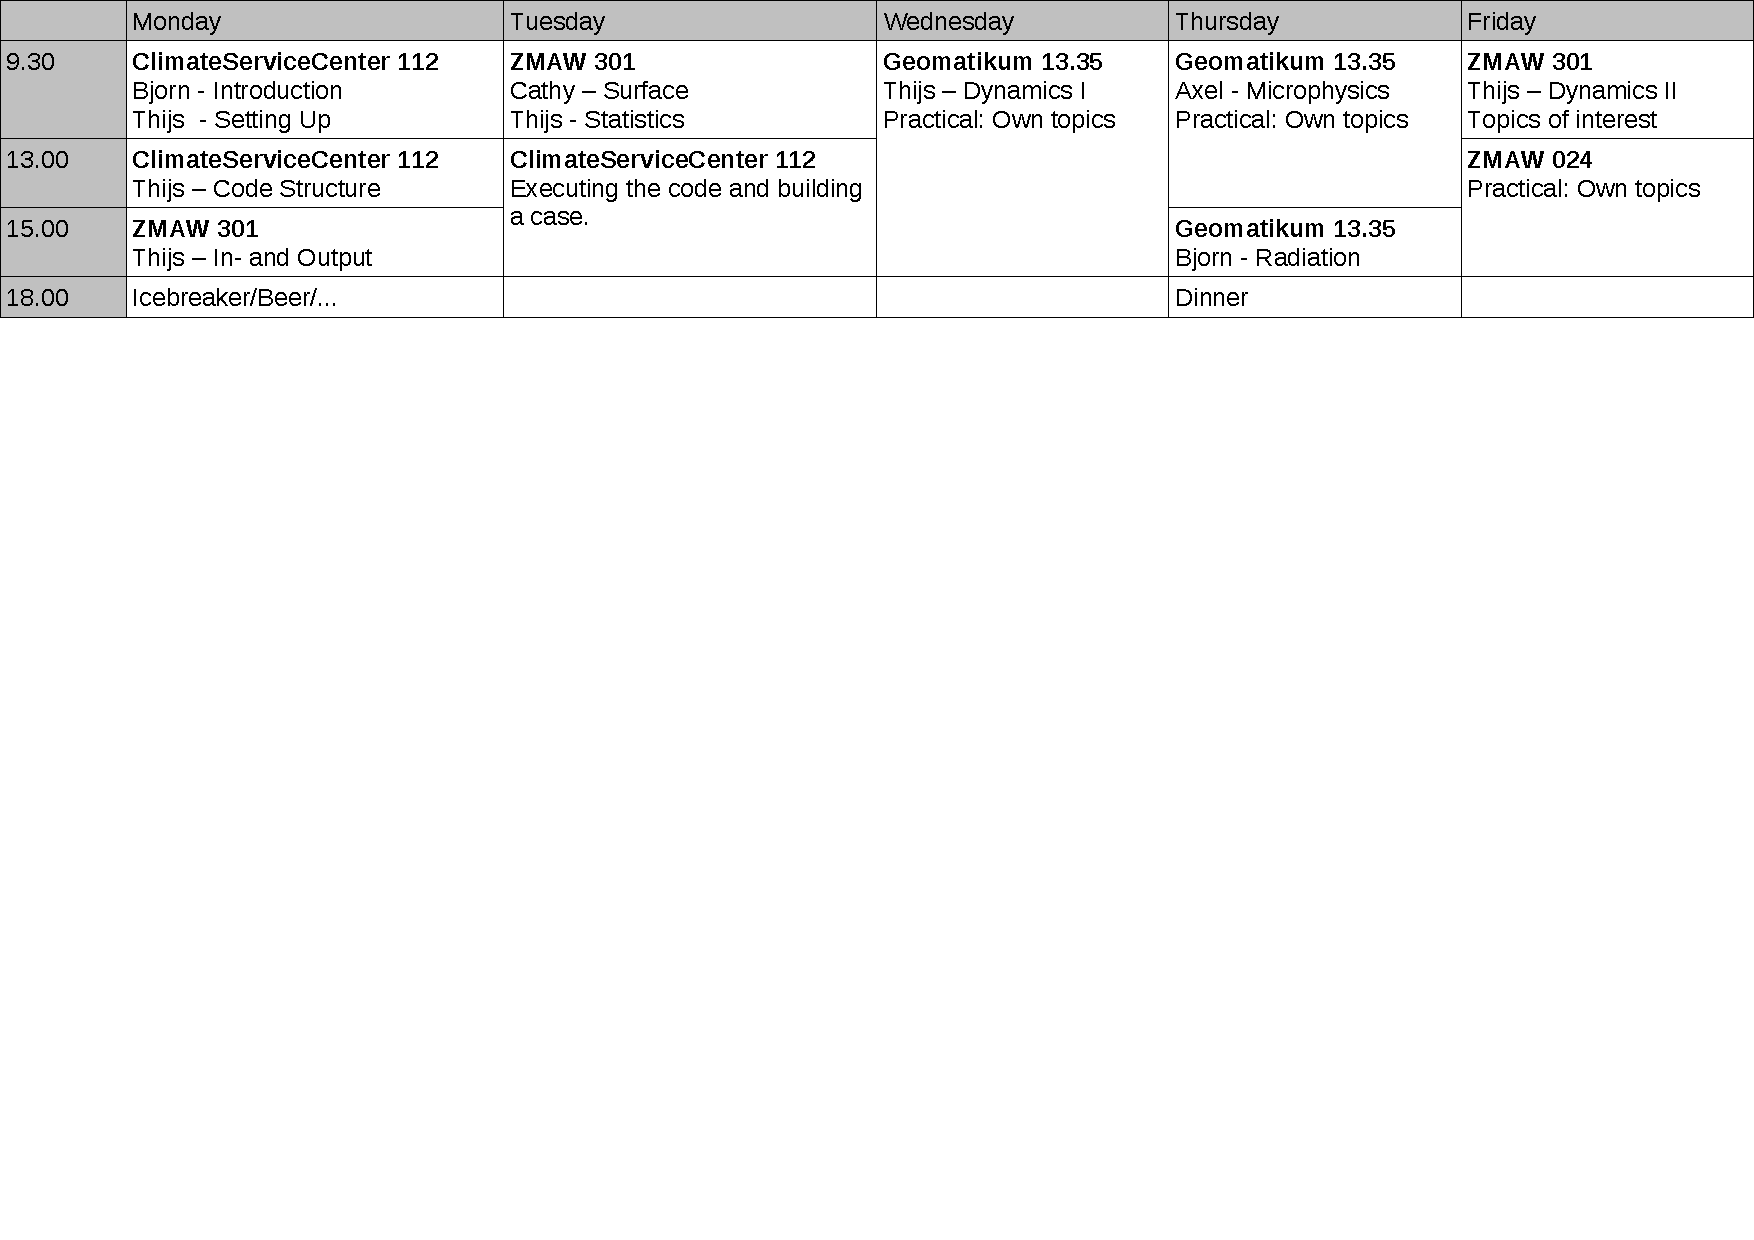
\includegraphics[width=\textwidth]{schedule.pdf}
\end{frame}
\begin{frame}{Our Group}
 \begin{itemize}
  \item Hans-Ertel Zentrum for research on Clouds and Convection
  \item Led by Cathy Hohenegger and Axel Seifert
  \item Funded by Deutscher Wetter Dienst
  \item Hunt for knowledge on convective clouds in various conditions
  \item Large Eddy Simulations are our primary (but not only) tool
 \end{itemize}

\end{frame}

\begin{frame}[<+->]{Cascade of Models}
 \begin{itemize}
  \item General Circulation Models
  \item Regional Models
  \item \alert{Large-Eddy Simulations}
  \item Direct Numerical Simulations
 \end{itemize}

\end{frame}
\begin{frame}[<+->]{Cascade of Models}
\framesubtitle{General Circulation Models}
\begin{itemize}
 \item Domain size: Entire Earth
 \item Horizontal Boundary conditions: None
 \item Horizontal grid spacing: $50 \mathrm{km}$
 \item Total number of points: about $400 \times 400 \times 100 $
 \item Simulation duration: Weeks - millennia
 \item Resolved: Hadley Circulation, fronts, ...
 \item Parameterized: Clouds,  Boundary layers, Surface, Microphysics
\end{itemize}
 
\end{frame}

\begin{frame}{Cascade of Models}
\framesubtitle{Regional Models}
\begin{itemize}
 \item Domain size: Continental scale or smaller
 \item Studies of organization, deep systems,...
 \item Horizontal Boundary conditions: Nested/forced by GCM
 \item Horizontal grid spacing: $5 \mathrm{km}$
 \item Total number of points: about $400 \times 400 \times 100 $
 \item Simulation duration: Weeks
 \item Resolved: Deep clouds
 \item Parameterized: Shallow Clouds,  Boundary layers, Surface, Microphysics
\end{itemize}
 
\end{frame}
\begin{frame}{Cascade of Models}
\framesubtitle{Large-Eddy Simulations}
\begin{itemize}
 \item Domain size:$1 - 100\mathrm{km}$
 \item Studies of boundary layer processes, idealized (and not so idealized) clouds
 \item Horizontal Boundary conditions: Periodic
 \item Horizontal grid spacing: $50 \mathrm{m}$
 \item Total number of points: about $400 \times 400 \times 100 $
 \item Simulation duration: Hours/Days
 \item Resolved: Shallow Clouds,  Boundary layers
 \item Parameterized: Turbulence, Surface, Microphysics
\end{itemize}
 
\end{frame}

\begin{frame}{Cascade of Models}
\framesubtitle{Direct Numerical Simulations}
\begin{itemize}
 \item Domain size:$1\mathrm{m}$
 \item Studies of turbulence, possibly with interactions of other processes
 \item Horizontal Boundary conditions: Periodic
 \item Horizontal grid spacing: $1 \mathrm{mm}$
 \item Total number of points: about $1000 \times 1000 \times 1000 $
 \item Simulation duration: Minutes
 \item Resolved: Turbulence, surface (?)
 \item Parameterized: Microphysics
\end{itemize}
 
\end{frame}
\begin{frame}{Cascade of Models}
\framesubtitle{Other}
Focus of LES is on Geophysical \emph{Fluid Dynamics}

Many processes are still unresolved or beyond the scope of LES:
\begin{itemize}
 \item Radiation - At best, 2D radiation is available
 \item Chemistry, aerosols and microphysics
 \item Near-Surface processes
\end{itemize}
\end{frame}

\section{Large-Eddy Simulations}
\begin{frame}[<+->]{Large-Eddy Simulations}
\framesubtitle{Principle}
 \begin{itemize}
  \item Spatially filter (smooth) the Navier Stokes Equations
  \item Ensure that the width of this spatial filter lies in the inertial subrange of the turbulent field
  \item Explicitly solve the most energetic scales
  \item Model the Sub Filter Scale (SFS) turbulence. The details of this SFS model should not matter. 
 \end{itemize}
We violate these principles on a daily basis. But still, over $90\%$ of the energy in the bulk of the convective boundary layer is usually resolved.

\end{frame}

\begin{frame}{Filtering}

\[
 \bar{u} = \int G(r) u \mathrm{dr}
\]
 With $G$ the filter (could be a (grid-)box, a gaussian, a spectral filter,....)
\end{frame}

\begin{frame}{Navier Stokes Equations}
 \begin{align*}
\frac{\partial {u}_i}{\partial t} & = 
&{- {u}_j \frac{\partial {u}_i}{\partial x_j} }
&{- c_p \Theta_0 \frac{\partial{\pi}}{\partial x_i}}
&{+ \nu \frac{\partial^2 u_i} {\partial x^2_j}}
&{ + \force{i}{} }
\end{align*}

\end{frame}

\begin{frame}{Large-Eddy Equations}
 \begin{align*}
\frac{\partial \bar{u}_i}{\partial t} & = 
&{- \bar{u}_j \frac{\partial \bar{u}_i}{\partial x_j} }
&{- c_p \Theta_0 \frac{\partial\bar{\pi}}{\partial x_i}}
&{+ \frac{1}{\rho_0} \frac{\partial (\rho_0 \tau_{ij})} {\partial x_j}}
&{ + \force{i}{} }
\\
\frac{\partial \bar{\phi}}{\partial t} & = 
&{ - \bar{u}_j \frac{\partial  \bar{\phi}}{\partial x_j}} 
&&{+ \frac{1}{\rho_0} \frac{\partial (\rho_0  \gamma_{\phi j})} {\partial x_j}}
&{+\source{\phi}{}}
\end{align*}
{
Anelastic continuity $$
 \frac{\partial (\rho_0 u_i) }{\partial x_i} = 0 \label{eq:continuity}
$$
}
{
Ideal gas law equation of state $$\theta_v = \theta\left(1 + (R_v/R_d-1)q_t - (R_v/R_d)q_l\right).$$
}

\end{frame}

\begin{frame}{Closure}
 \begin{itemize}
  \item $\tau_{ij} \equiv \overline{u_i u_j} - \bar{u}_i \bar{u}_j $ is the Sub Filter Scale flux and needs to be modeled
  \item Can be done by
  \begin{itemize}
   \item Smagorinsky diagnostic closure
   \item Deardorff prognostic TKE
   \item Higher order closures
   \item Nothing at all (Numerical diffusion)
  \end{itemize}
  \item All models start off with models for homogeneous isotropic turbulence 
  \item Empirical modifications are nearly always done to match stable turbulence and condensation gradients.
 \end{itemize}
\end{frame}
\section{History}
 
\begin{frame}{History}
 \begin{itemize}
  \item Dry LES: Smagorinsky (1963), Lilly(1967), Deardorff(1972)
  \item Cloudy LES: Sommeria(1976)
  \item 'Big breakthrough LES': Schmidt and Schumann (1989)
  \item 'Huge breakthrough LES': Earth Simulator Global LES (2001) 
 \end{itemize}

\end{frame}

\begin{frame}[allowframebreaks]{History}
\framesubtitle{Intercomparisons}
\begin{itemize}
 \item \alert{Dry CBL}:  Nieuwstadt et al. (1986, 1993) and Andren et al. (1994)
 \item \alert{Non-Precip Stratocumlus}: Moeng et al. (1996)
 \item \alert{Radiative Smoke}: Bretherton et al. (1999)
 \item \alert{Non-Precip Shallow Cu}: Siebesma et al. (2003)
 \item \alert{Non-Precip Stratocumlus}: Stevens et al. (2001)
 \item \alert{Diurnal Cycle Cu}: Brown et al. (2001)
 \item \alert{Sheared and Stable BLs}: Holtslag(2006), Beare(2006)
 \item \alert{Precip Stratocumlus}: Ackerman et al. (2008)
 \item \alert{Precip Cumlus}: van Zanten et al. (2011)
 \item \alert{Precip Stratocumlus}: Ackerman et al. (2008)
 \item \alert{Radiative, transition runs}: Sandu, de Roode, Blossey (2012)
\end{itemize}
 
\end{frame}

\begin{frame}{History}
\framesubtitle{UCLALES}
 \begin{itemize}
  \item Based on a meso-scale modeling code by prof. Cotton and prof. Pielke at Colorado State University  (eighties, nineties)
  \item Started as LES by Bjorn in the nineties
  \item Blossomed with him at UCLA (hence the name)
  \item Parallelized by Jim Edwards, Microphysics with help of Graham Feingold and Axel Seifert, dynamics by Verica Savic Jovcic
  \item Participated in all GCSS intercomparisons, and in many process studies
 \end{itemize}

\end{frame}

\begin{frame}[<+->]{When \emph{not} to use LES}
 When your problem has ...
\begin{itemize}
 \item ... nothing to do with turbulence
 \item ... exclusively to do with turbulence (use DNS!)
 \item ... is dominated by larger scales (e.g. frontal systems)
\end{itemize}
Or when you don't have sufficient computer power to do high resolution simulations. In which case, start doing theory.
\end{frame}
\begin{frame}[<+->]{When not (yet) to use \emph{UCLA LES}}
 When your problem has ...
\begin{itemize}
 \item ... strong pressure fluctuations (anelastic approximation is used)
 \item ... orography, heterogeneous surface conditions or land-atmosphere interactions
 \item ... has an important lateral component to it (Periodic boundary conditins)
\end{itemize}
Or when you're not willing to look into the code.
\end{frame}
\begin{frame}{What \emph{can} be done with (UCLA) LES}
\framesubtitle{Classical studies}
\begin{itemize}
 \item Clear convective boundary layers
 \item Shallow cumulus clouds
 \item Stratocumulus clouds
\end{itemize}
 
\end{frame}
 \begin{frame}
  {What \emph{can} be done with (UCLA) LES}
\framesubtitle{Modern studies}
\begin{itemize}
 \item Precipitation and microphysics
 \item Cloud and parcel tracking
 \item Deep convection
 \item Stable boundary layers
 \item Surface interaction
 \item Day-to-day runs like in the KNMI Testbed
\end{itemize}
 
 \end{frame}

\begin{frame}{Model Philosophy}
Why use stand-alone LES models at all?
\begin{itemize}
 \item Research desires ad-hoc changes
 \item Big model structures (WRF, ECHAM, ICON...) tend to be cluttered, lots of unnecessary additions, hard to run and compile, unreadable,...
 \item UCLALES is just small enough to understand (more or less)
 \item It is easy to code any forcing/output you want, and use it for 1 study
 \item Optimized for user/developer time, not CPU Time
\end{itemize}
 \end{frame}
\begin{frame}{Course Aim}
 After this course, you should...
\begin{itemize}
 \item Be able to run and tweak the model
 \item Know where to look up scripts and examples (including in these handouts)
 \item Understand the (im-)possibilities and sensitivities of UCLA LES
 \item Have a feel for what resolution should be used when, and what model setting is necessary.
\end{itemize}

\end{frame}
\begin{frame}{Drinks tonight?}
\begin{center}
\huge{Hadley's, 18.00?} \end{center}
\end{frame}
